% 0519 修改
% 背景介绍:随着RBS的结构复杂度的增长,特别是当有电池隔离的情况出现,人工MAC判断越来也困难,需要具有普适性的算法
% 模型:保留电路模型的相关推导;旧版两个图统一为一个拓扑模型图 topologic model
% 讨论:电池组拓扑设计新思路,新的复杂结构(仅作验证);电池隔离(尽量写)
% 保留电路模型的相关推导
% 图片:重画所有图,用ppt,注意字体大小、元素含义统一
% 专有名词的统一:structure, external electrical appliance, components
% 伪代码:修改后放附录





\documentclass{article}
\usepackage{graphicx}
\usepackage{subcaption}
\usepackage{enumerate}
\usepackage{amsmath}
\usepackage{multirow}
\usepackage{bm}
\usepackage[ruled,linesnumbered]{algorithm2e}

\def\T{\mathrm{T}}


\title{A Greedy-based calculation method of RBS maximum allowable current}
\author{3057761608 }

\begin{document}

\maketitle

\begin{abstract}
    Reconfigurable Battery Systems (RBSs) offer a promising alternative to traditional battery systems owing to their dynamical topologic structure for the optimization of battery cell charging and discharging stragegies.
    During the operation of the RBS, the Maximum Allowable Current (MAC) is a critical indicator to guide the reconfiguring control of the system in terms of safety and reliability.
    In this paper, the MAC of the RBS is calculated by using a greedy algorithm based on the topologic model of the RBS.
    The effectiveness of this method is validated on the RBSs with different structures.
    % #TODO


    keywords: Reconfigurable Battery System, Maximum Allowable Current, Greedy Algorithm
\end{abstract}

\section{Introduction}

Battery Energy Storage Systems (BESSs) are widely used to store and supply high-quality electrical energy in various applications, such as smart grids and wind power plants \cite{desiqueiraControlStrategySmooth2021,karandehTwoStageAlgorithmOptimal2019,yangBatteryEnergyStorage2018,choCommercialResearchBattery2015}.
Typically, a BESS consists of numerous battery cells that are interconnected by series-parallel circuitry to provide the required charge storage capacity and output voltage.
For the traditional BESS, the connections between batteries are fixed and the performance of system is limited by the worst cell, as the result of the cask effect.
Furthermore, reliability and even safety issues will alse be aroused since the failed battery cannot be promptly isolated to exacerbate the degradation of the other batteries during the operational process \cite{yangUnbalancedDischargingAging2016,fengPropagationMechanismsDiagnosis2019}.
Undoubtedly theses issues hinder the practical application of traditional BESSs.


Reconfigurable Battery System (RBS), which can dynamically switch to arbitrary circuit configurations as required, is expected to solve the above problem\cite{hanNextGenerationBatteryManagement2020a}. 
The ability to switches circuit helps to isolate unhealthy batteries from the circuit in a timely manner, thereby improving the safety and reliability of the battery system.
Fig. \ref{fig:arch} shows two popular typologies of the RBSs developed by Lawson\cite{lawsonSoftwareConfigurableBattery2012} and Visairo \cite{visairoReconfigurableBatteryPack2008} respectively. 
Taking the RBS shown in Fig. \ref{fig:arch-e} as example, the batteries in the RBS can beare connected not only in series when the switches $S_1$, $S_5$, $S_6$, $S_7$, $S_8$, $S_9$, and $S_{13}$ are closed, but also in parallel when $S_1$, $S_2$, $S_3$, $S_4$, $S_5$, $S_9$, $S_{10}$, $S_{11}$, $S_{12}$, and $S_{13}$ are closed.
Furthermore, when an unhealthy battery, for instance the orange one in Fig. \ref{fig:arch-f}, exits in the RBS, it can be isolated by closing its three adjacent switches (i.e. $S_5$, $S_7$ and $S_8$) and opening the switch below that battery (i.e. $S_6$) to ensure the system still remains a reliable working mode.

\begin{figure}[htbp]
    \centering
    \begin{subfigure}[b]{0.15\textwidth}
        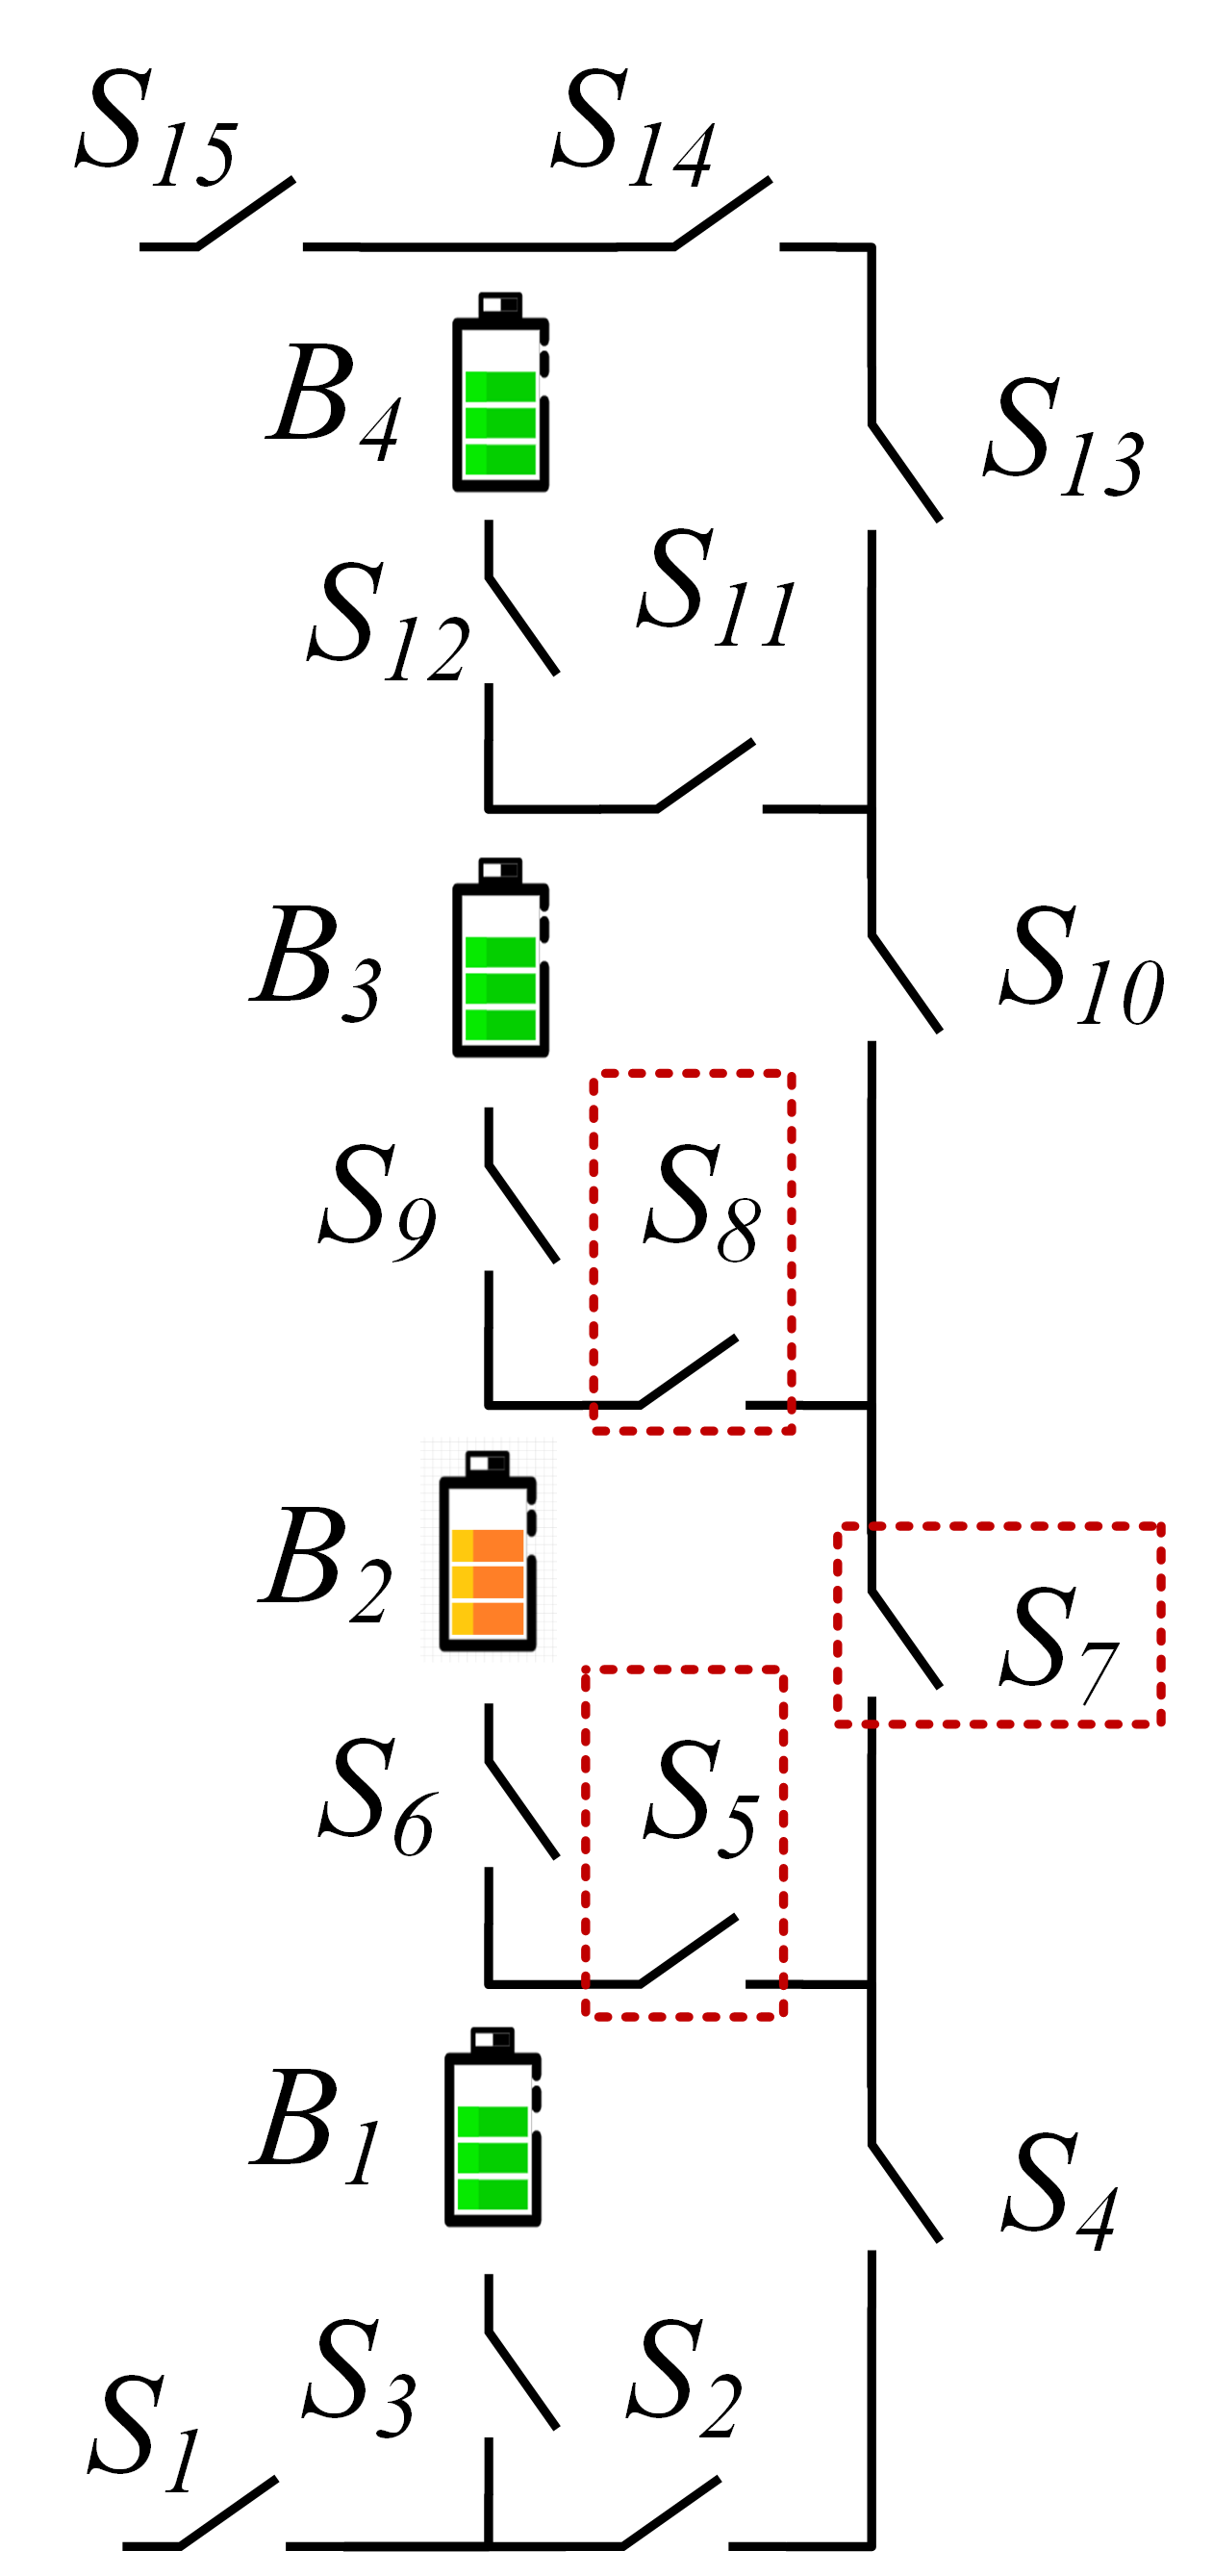
\includegraphics[width=\textwidth]{../attachments/arch-e.png}
        \caption{}
        \label{fig:arch-f}
    \end{subfigure}
    \hspace{0.05\textwidth}
    \begin{subfigure}[b]{0.45\textwidth}
        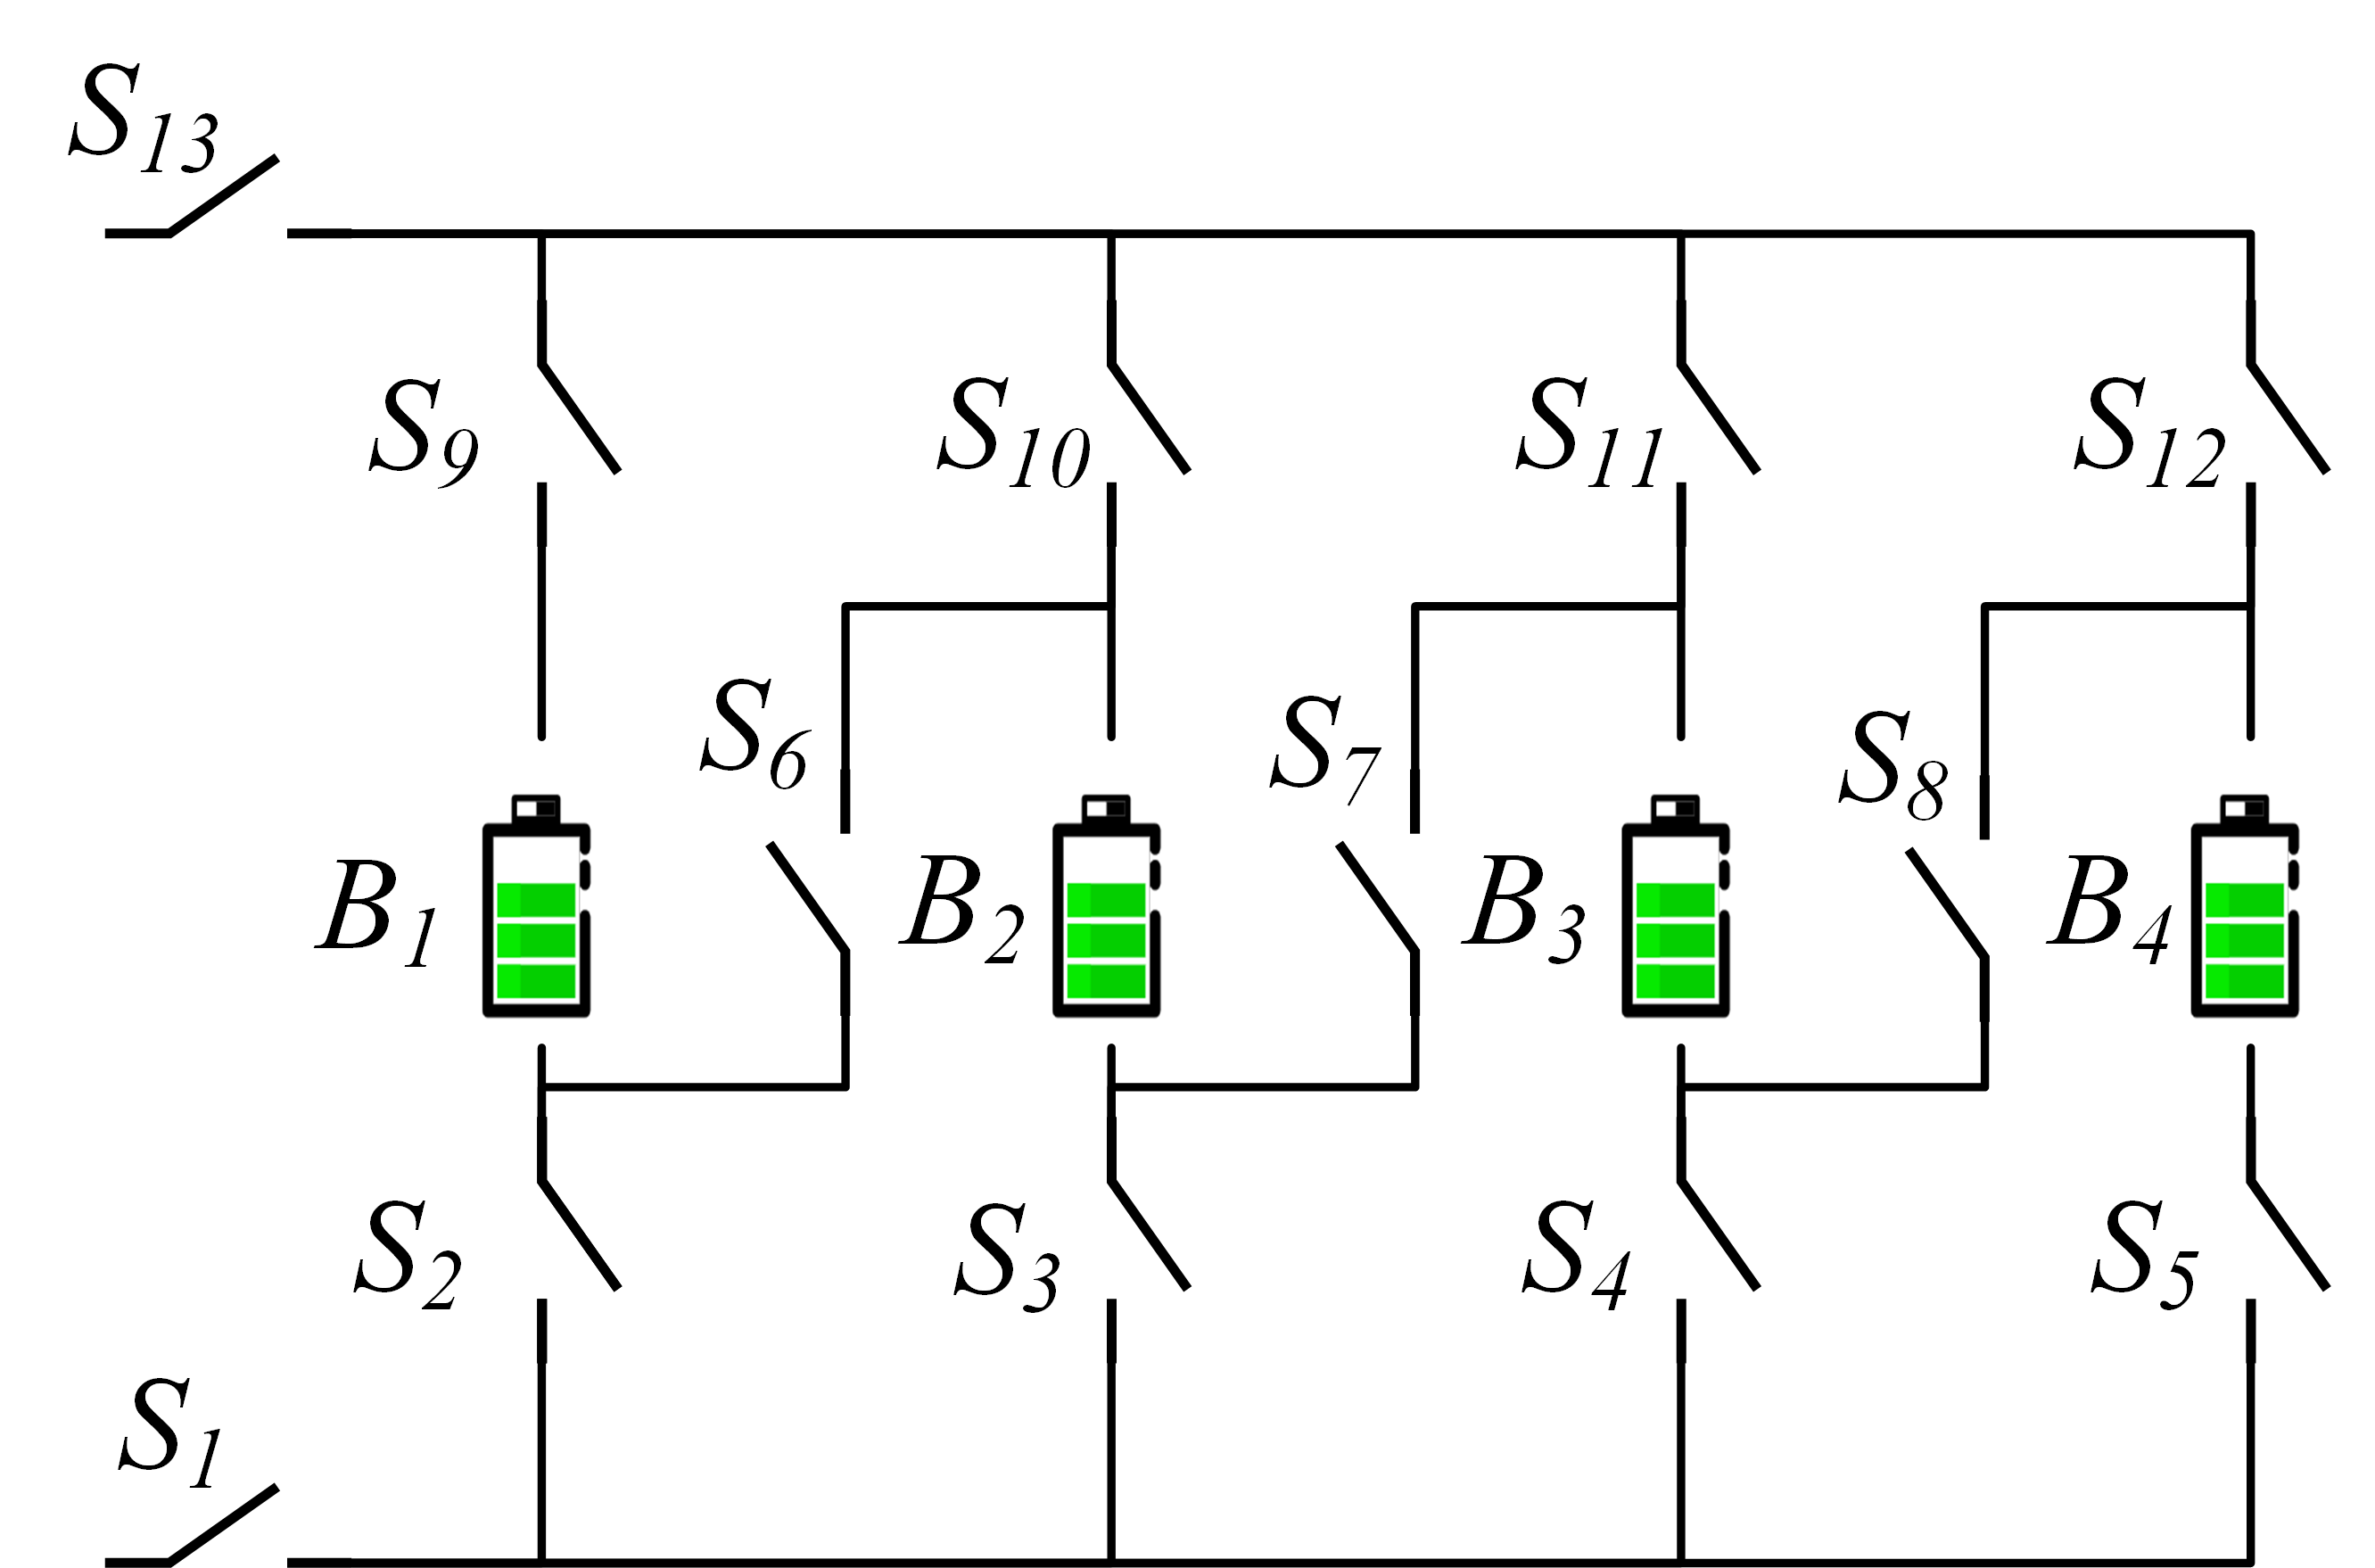
\includegraphics[width=\textwidth]{../attachments/arch-f.png}
        \caption{}
        \label{fig:arch-e}
    \end{subfigure}
    \caption{The RBS structure proposed by (a)Lawson\cite{lawsonSoftwareConfigurableBattery2012}, (b)Visairo\cite{visairoReconfigurableBatteryPack2008}.}
    \label{fig:arch}
\end{figure}

The complex connecting structure between batteries and switches enables the flexibility of the RBS, but also brings the challenges in design and control cost.
The Maximum Allowable Current (MAC) of the RBS system is defined as the maximum current that is allowed for each individual battery of the system, and is a critical indictor to be evaluate the RBS output current to the electronic appliances.
It helps the designer to assess whether the RBS meets the output current requirements, and contributes to the formulation of appropriate and safe management stragegies for the battery management system (BMS).
As the complexity of RBS increases, especially when the certain battery needs to be isolated, it becomes difficult to visually obtain the MAC, and a universal algorithm is needed to solve the MAC.
Despite its importance, there is currently no method available to evaluate MAC for RBSs.
Therefore, the purpose of this paper is to propose a universal and effective method for calculating the MAC of the RBS.
To achieve this, a topologic model that builds the relationship between RBS circuit topology and internal resistance and voltage of its batteries are established.
Then, a greedy algorithm is employed to search the available circuit of the RBS for reaching the MAC.
With the developed method, MAC of RBSs with different structures can be calculated effectively.


The remainder of this paper is organized as follows:
Section II presents the framework and details of the proposed topologic model and the greedy algorithm.
In Section III, a case study of using the proposed model and algorithm to enumerate the MAC of a specific structure is demonstrated.
Finally, the concluding remarks are drawn in Section IV.


\section{Methodology}

The overall MAC modeling process from an RBS structure is shown in Fig. \ref{fig:main}, which can be divided into four main steps.
In the first place, the actual RBS structure is converted to a topologic model, in which the connected relationships between batteries and switches are abstracted and the performance parameters of the batteries are retained.
Subsequently, constraints and objective function, i.e. MAC, are obtained based on the previous connected relationships and parameters.
Then, the shortest path (SP) of each battery in the RBS is obtained by Dijkstra algorithm.
In the end, the open/close strategy of the RBS is implemented by greedily selecting the SPs to achieve MAC and quantitatively calculated in the equivalent circuit.
% 只有一个 topologic model,建模;先根据连接关系和物理参数建立目标函数和约束;再找SP;最后根据贪婪算法求解MAC。

% TODO: fig 整体框图
\begin{figure}
    \centering
    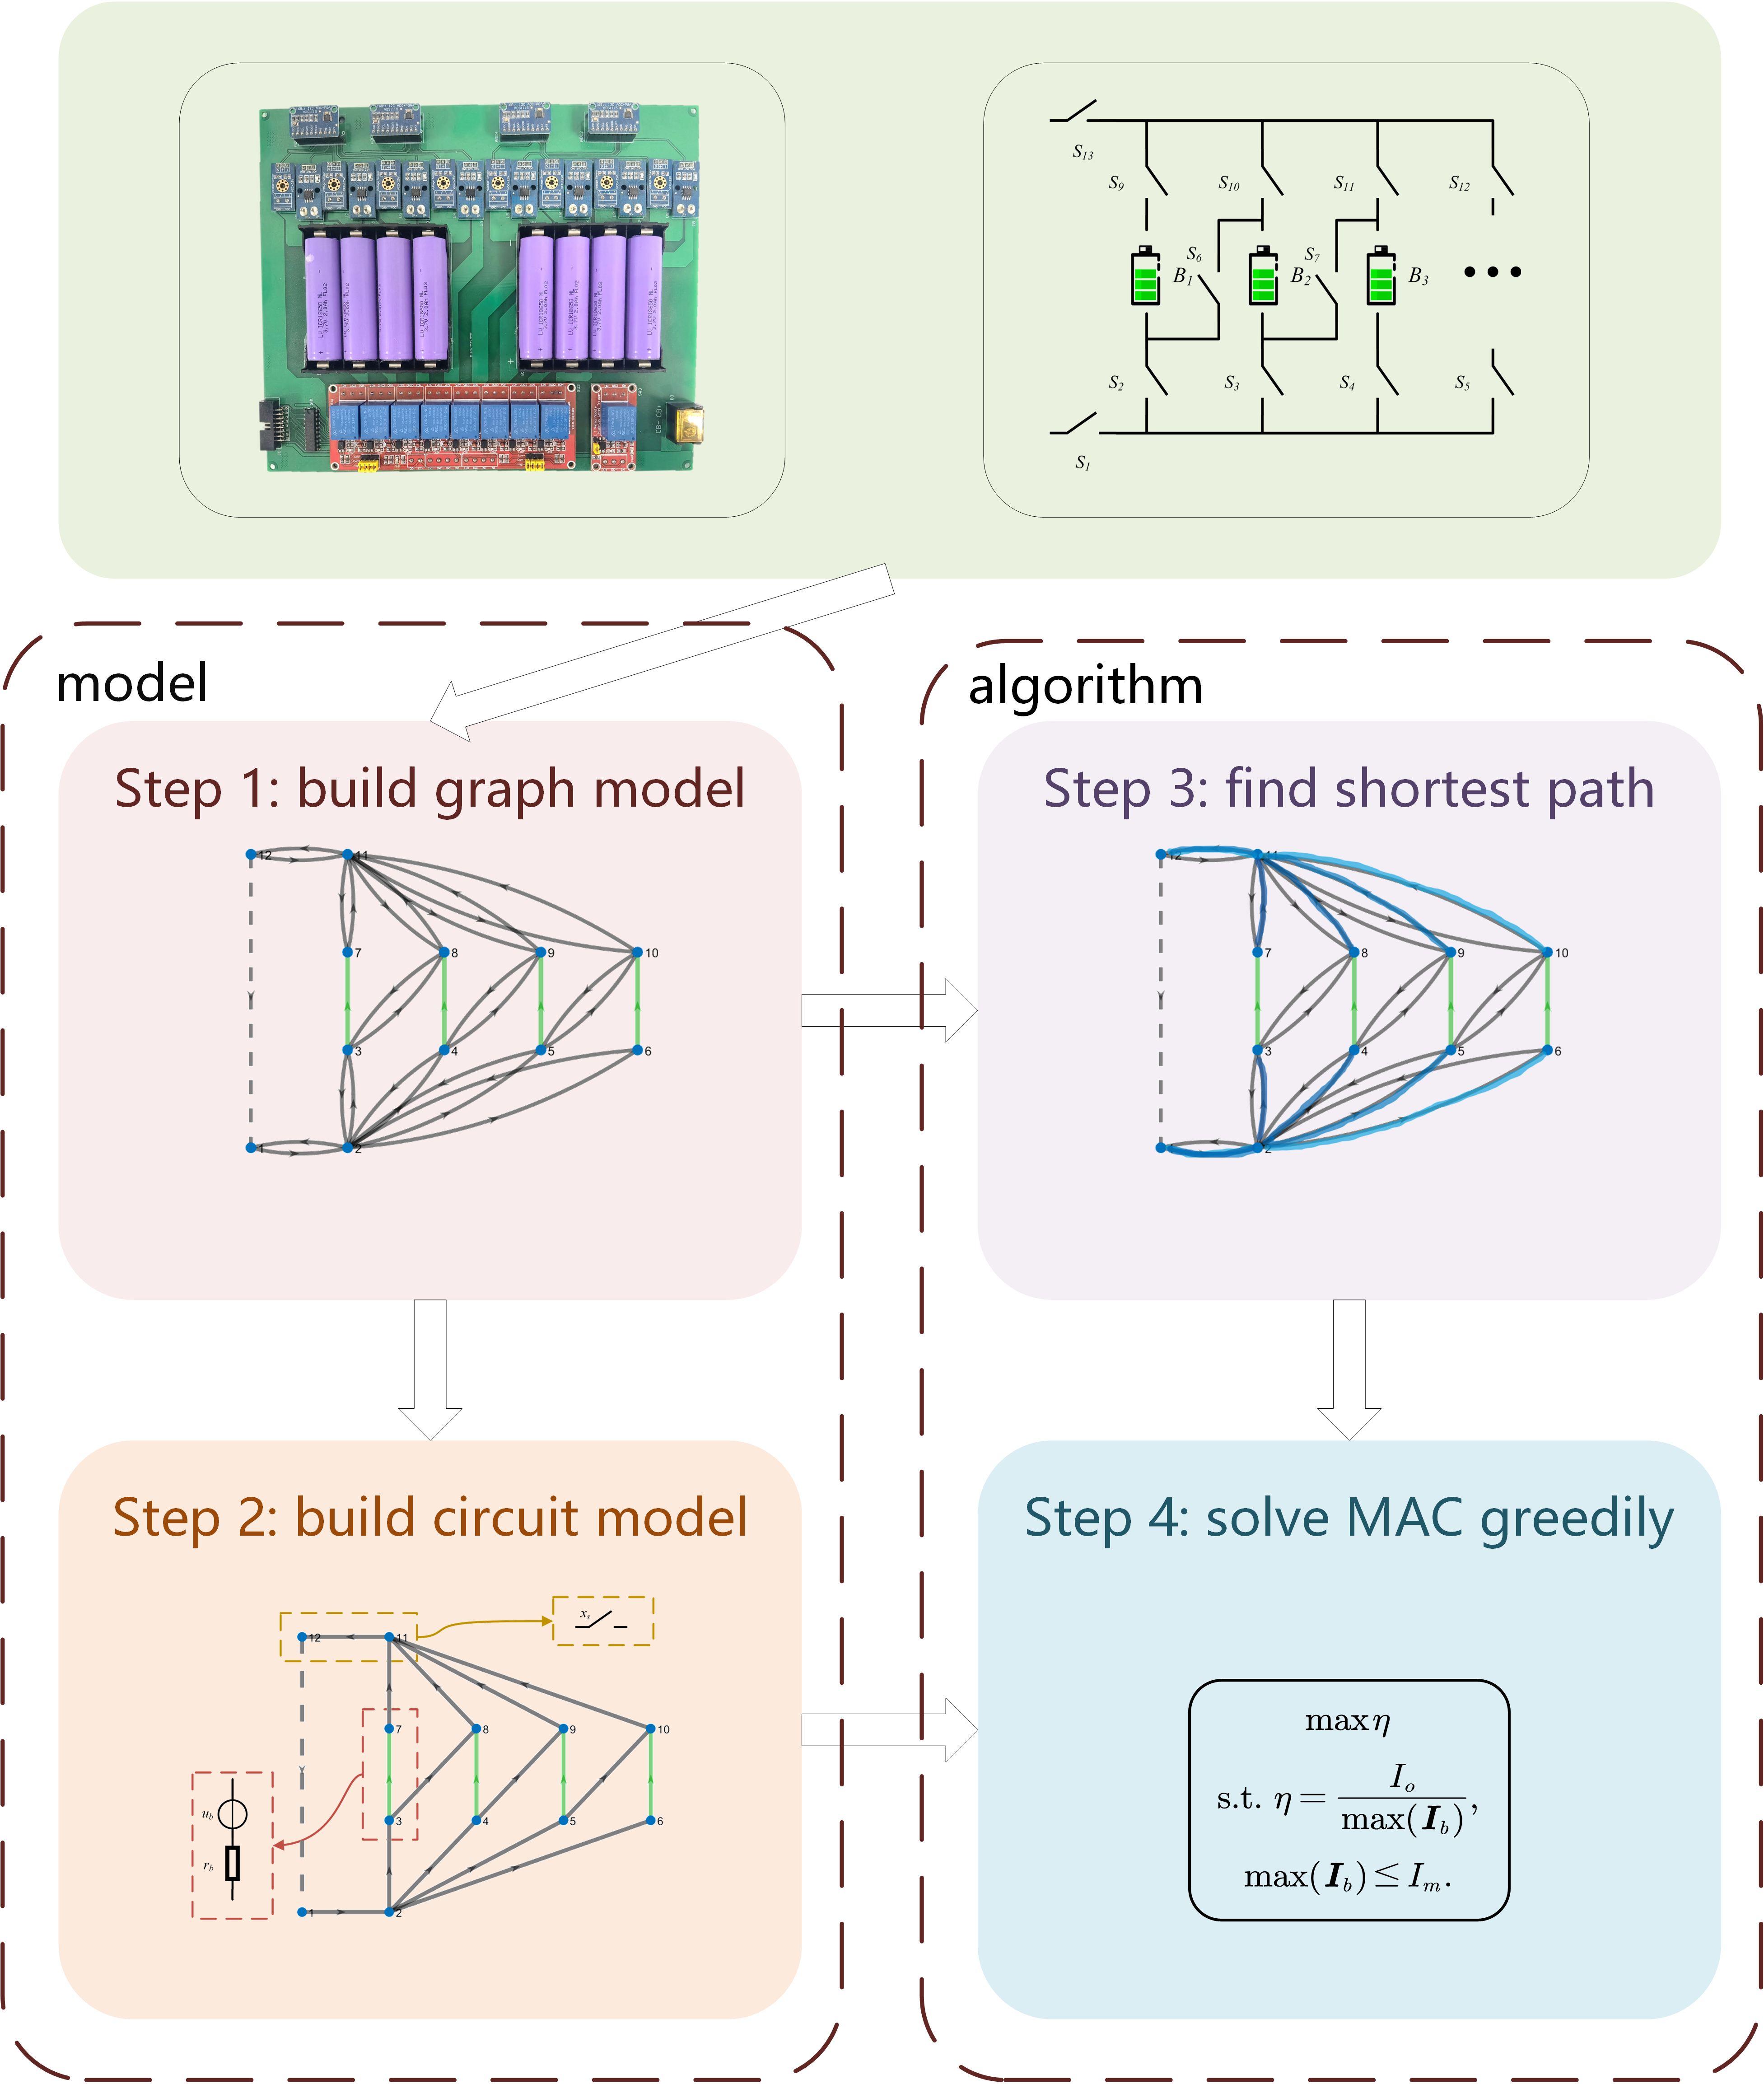
\includegraphics[width=\textwidth]{../attachments/main-v4.png}
    \caption{Diagram of this method. 
        It includes a graph model and an equivalent circuit model based on the actual RBS.
        The shortest path of each battery is obstained from the graph model, and the voltage and current of the equivalent circuit model are calculated.
        By greedily searching for the combination of the shortest path, the MAC is calculated in the equivalent circuit model.
        } 
    \label{fig:main}
\end{figure}

\subsection{Topologic Model}

As demonstrated in Fig. \ref{fig:arch}, a typical RBS is made up of a number of battery cells and switches in a dynamically adjustable connection.
To establish a processable circuit, these batteries and switches are transformed into ideal elements under reasonable assumptions.
The resulting circuit structure is then described in matrix form, and the related equations are provided.


The normal equivalent circuit for a battery consists of a voltage source in series with a resistor, and a capacitor in parallel with another resistor to simulate the polarization in batteries.
To simplify the model, the transient characteristics of the circuit are not considered, so the capacitor mentioned above is ignored.
In this way, the battery $i$ in the RBS is modeled by the series connection in between a constant voltage source $u_{b,i}$ and a resistor $r_{b,i}$,  as shown in Fig. %TODO 电池模型有电阻电容简化为电阻的示意图。
And a binary variable $x_j$ is used to represent the state of switch $j$, where 0 for ON and 1 for OFF, respectively.
To simplify the calculation, a closed switch is considered as a resistor with a very small resistance value $r_s$.


For a given RBS structure, the topologic model for the RBS is constructed as a directed graph $G(V,E)$ in such a way that:
\begin{enumerate}
    \item Nodes: node $v_1$ and $v_N$ represent the anode and cathode of the RBS respectively, and the other nodes $v_2,\cdots , v_{N-1}$ represent the points connecting batteries and/or switches, where $N$ is the total number of nodes.
    \item Edges: the directed edges represent batteries, switches and the external electrical appliance in the output circuit based on whether the current direction is constrainted or not. 
        When the battery is in operation, the internal current direction must be from the negative electrode to the positive electrode, so it is represented by a directed edge from the negative to the positive ; this edge has attributes $(u_b, r_b)$, where $u_b$ and $r_b$ represent battery $b$'s electromotive force and internal resistance.
        Switches have no constraints on the current direction, so they are represented by a pair of directed edges with opposite directions; these edges both have attribute $(0, r_s)$, where $r_s$ represents the resistance of switch as mentioned above.
        To fully solve for the current and voltage, an external electrical appliance equivalent as a resistor $R_0$ is connected to the anode and cathode of the RBS and represented by a directed edge from the anode $v_N$  to the cathode $v_1$ of the RBS.
        Similarly, this edge has attribute $(0, R_0)$.
        If a given RBS structure has $N_b$ batteries and $N_s$ switches in total, then the number of edges is $N_b+2N_s+1$, where 1 refers to the external electrical appliance.
\end{enumerate}

\subsection{Constraints and Objective Function}

The constraints and objective function are obtained by analyzing the currents of batteries and external electrical appliance, as following.
Based on the above directed graph which has $N$ nodes and $N_b+2N_s+1$ directed edges, its incidence matrix $\bm{A}$ is defined as
\begin{align}\label{eq:A}
    $a_{ij}$=
    \begin{cases}
        1,  & \text{edge  $j$ leaves vertex $i$},\\
        -1, & \text{edge $j$ enters vertex $i$},\\
        0,  & \text{otherwise}.
    \end{cases}
\end{align}
Since each column of $\bm{A}$ sums to zero, the last line are deleted.
Furthermore, because of a couple of opposite directed edges for each switch, the $N_s$ columns corresponding to the switches are also deleted.
Finally, the reduced incidence matrix $\bm{A}_{(N-1)\times(N_b+N_s+1)}$ are used in the following calculation.
By divided as batteries, switches and external electrical appliance, $A$ is rewritten as follows
\begin{equation}
    \bm{A} =
    \begin{bmatrix}
        \bm{A}_b & \bm{A}_s & \bm{A}_o
    \end{bmatrix}.
\end{equation}


$N_b+N_s+1$ edges' currents $\bm{I}_{(N_b+N_s+1)\times 1}$ and voltages $\bm{U}_{(N_b+N_s+1)\times 1}$, and $N-1$ nodes' voltages $\bm{U}_{n, (N-1)\times 1}$ have following relationships from Kirchhoffs law
\begin{align}\label{eq:Kirchhoffs_law}
    \begin{cases}
        $\bm{A} \bm{I} = \bm{0}$, \\
        $\bm{U}        = \bm{A}^\T \bm{U}_n.$
    \end{cases}
\end{align}
These directed edges are treated as generalized branches and expressed in matrix form as follows
\begin{equation}\label{eq:generalized_branches}
    \bm{I} = \bm{Y}\bm{X} \bm{U} - \bm{Y}\bm{X} \bm{U}_s +\bm{I}_s,
\end{equation}
where $\bm{I}$ and $\bm{U}$ are the column vectors about $1+N_b+N_s$ edges' current and voltage, respectively;
$\bm{U}_s$ and $\bm{I}_s$ denote the source voltage and source current of the generalized branches, respectively;
$\bm{Y}$ is the admittance matrix of the circuit, and $\bm{X}$ is the state matrix defined as
\begin{equation}\label{eq:X}
    \bm{X} = \diag(
    \underbrace{1, \cdots, 1}_{N_b~\text{of}~1},
    \underbrace{1, 0 \cdots, 1}_{N_s~\text{of}~0/1},
    1)
    =\begin{bmatrix}
        \bm{X}_s &\\
        & \bm{I}
    \end{bmatrix}.
\end{equation}


In addition to the equivalent circuit assumptions, we also assume that all batteries have the same internal resistance value $r_b$ and supply the same electric potential $u_s$ to simplify the model.
Then the output current $I_o$ and each battery's current $\bm{I}_b$ can be given by solving the simultaneous Eq. \ref{eq:Kirchhoffs_law} and \ref{eq:generalized_branches} eventually.
Let
\begin{equation}\label{eq:Yn}
    \bm{Y}_n (\bm{X}) = \frac{1}{R_o} \bm{A}_o\bm{A}_o^\T + \frac{1}{r_b} \bm{A}_b\bm{A}_b^\T + \frac{1}{r_s}\bm{A}_s\bm{X}_s\bm{A}_s^\T,
\end{equation}
where $R_o$ is the equivalent resistance of the external circuit.
Then, if $\bm{Y}_n$ is an invertible matrix,
\begin{align}
    I_o(\bm{X})      & = \frac{u_b}{R_o r_b} \bm{A}_o^\T \bm{Y}_n^{-1}(\bm{X}) \bm{A}_b \bm{I}_{N_b\times 1};\label{eq:I_o}\\
    \bm{I}_b(\bm{X}) & = \frac{u_b}{r_b^2}[\bm{A}_b^\T \bm{Y}_n^{-1}(\bm{X}) \bm{A}_b\bm{I}_{N_b \times 1}  -r_b \bm{I}_{N_b \times 1}],\label{eq:I_b}
\end{align}
where $\bm{I}_{N_b\times 1}$ is a column vector with all equal to 1.


In this study, the ratio of $I_o$ and $\max (\bm{I}_b)$ is used to characterize the maximum allowable current for a given RBS architecture, denoted as $\eta$:
\begin{equation}\label{eq:eta}
    \eta = \frac{I_o}{\max (\bm{I}_b)}.
\end{equation}
The discussion in the next section will show that the $\eta$ reflects the ability of the RBS architecture itself to deliver current, regardliess of the battery cells used by the RBS.
Finally the problem in RBS can be formulated as
\begin{align}\label{eq:max_eta}
    & \max \eta \label{eq:max_eta}\\
    & \max (\bm{I}_b) \leq I_m,
\end{align}
where $I_m$ is the maximum allowable current of the battery; $\eta$ can be calculated by Eq. \ref{eq:eta}; $I_o$ and $\bm{I}_b$ can be calculated by Eq. \ref{eq:I_o} and \ref{eq:I_b}.
However, it is computationally difficult to solve \ref{eq:max_eta} directly because of the presence of matrix $\bm{Y}_n^{-1}$.
As the number of batteries and switches in the RBS increase, the order of the matrix increases, and the time costed to compute increases sharply.
A greedy algorithm is proposed to solve this problem in the next subsection.


\subsection{Greedy Solution}

In this subsection, a greedy algorithm is proposed based on shortest paths ($SP$s), which is given here firstly.
When the battery $i$ is connected to the anode $v_1$ and the cathode $v_N$ of the RBS by the path $p$ in the graph model, the distance $\omega$ of $p$ is defined by the following equation:
\begin{equation}\label{eq:weight}
    \omega(p) = N_s \cdot n_b (p) + n_s (p),
\end{equation}
where $N_s$ is the total number of switches in the system; $n_b(p)$ and $n_s(p)$ are number of batteries and switches in the path $p$ respectively.
$SP_i$ is defined as the path with the minimum $\omega$ for battery $i$.
\begin{equation}
    SP_i = \argmin_{p \in P_i} \omega(p),
\end{equation}
where $P_i$ is the set of all paths from $v_1$ to $v_N$ and passed through the directed edge $i$ in the direction of it.
Specifically, the Dijkstra algorithm can be used to implement the $SP_i$.
According to the definition, $SP_i$ gives the simplest strategy by which the control of battery $i$ is achieved with a minimum of switches while minimizing the influence of other batteries.
From the perspective of series/parallel, the more batteries are connected into circuit via their $SP$s, the more batteries are connected in parallel.
Since batteries can provide more total output current when connected in parallel than in series, the algorithm greedily selects as many cells as possible to be connected into to the overall circuit via their $SP$s to obtain the MAC.
The dichotomy method is also performed to faster find the right number of $SP$s.

After finding the potential SPs combinations about the MAC, the state variable $\bm{X}_s$ of the switches can be determined, and the optimization problem \ref{eq:max_eta} can be solved using Eq. \ref{eq:eta}, \ref{eq:I_o} and \ref{eq:I_b}.
The overall flowchart is shown in Fig. \ref{fig:flowchart}, and the corresponding pseudo-code of the algorithm is shown in Algorithm \ref{alg:eta_RBS}.
% TODO 算法流程图

\section{Case Study}

This section verifies the effectiveness of the above model and algorithm on several structures.
Firstly, the detailed modeling and solving process of a specific RBS structure (proposed by \cite{visairoReconfigurableBatteryPack2008}) with four battery cells is given.
Then, the effectiveness is verified on RBSs with different structures and sizes.
This section also explains the advantages of using $\eta$ to characterize MAC.

\subsection{An specific example}

\begin{figure}[htbp]
    \centering
    \begin{subfigure}[b]{0.45\textwidth}
        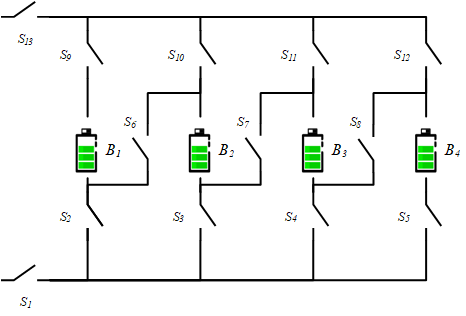
\includegraphics[width=\textwidth]{../attachments/f4-phy.png}
        \caption{}
        \label{fig:f4-phy}
    \end{subfigure}
    \hspace{0.05\textwidth}
    \begin{subfigure}[b]{0.45\textwidth}
        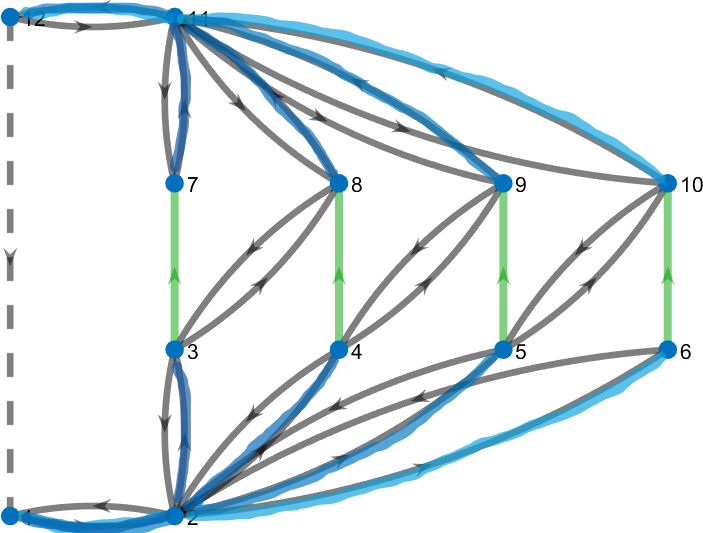
\includegraphics[width=\textwidth]{../attachments/v3-new-main-2.png}
        \caption{}
        \label{fig:f4-gra}
    \end{subfigure}
    \\
    \begin{subfigure}[b]{0.45\textwidth}
        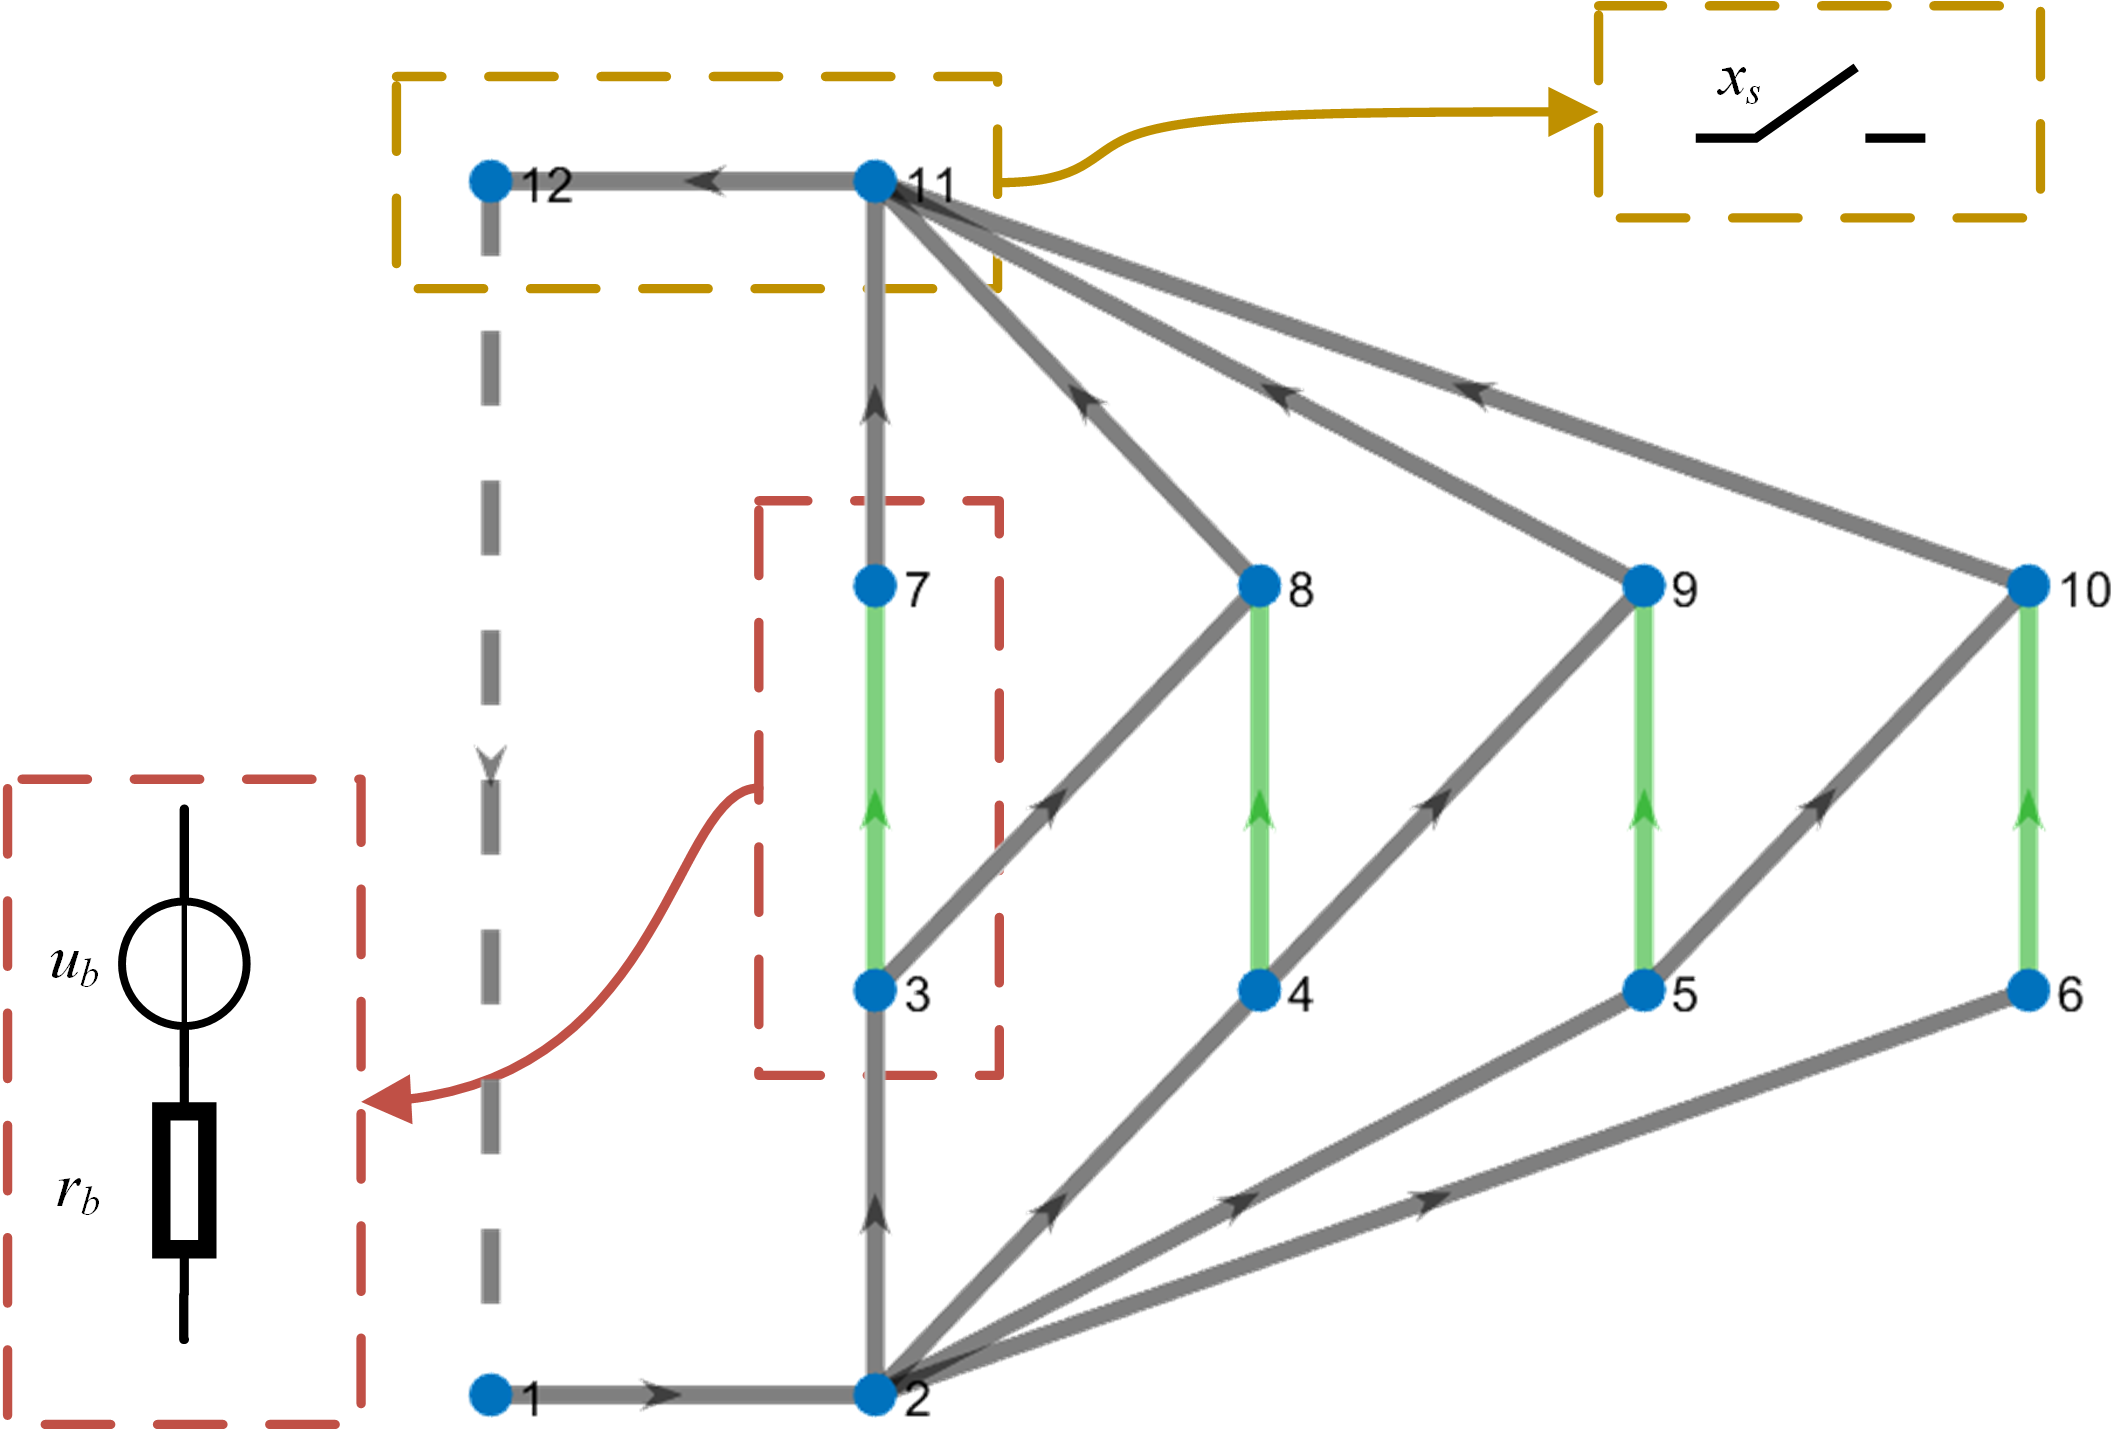
\includegraphics[width=\textwidth]{../attachments/f-dege-4-modify.png}
        \caption{}
        \label{fig:f4-circ}
    \end{subfigure}
    \hspace{0.05\textwidth}
    \begin{subfigure}[b]{0.45\textwidth}
        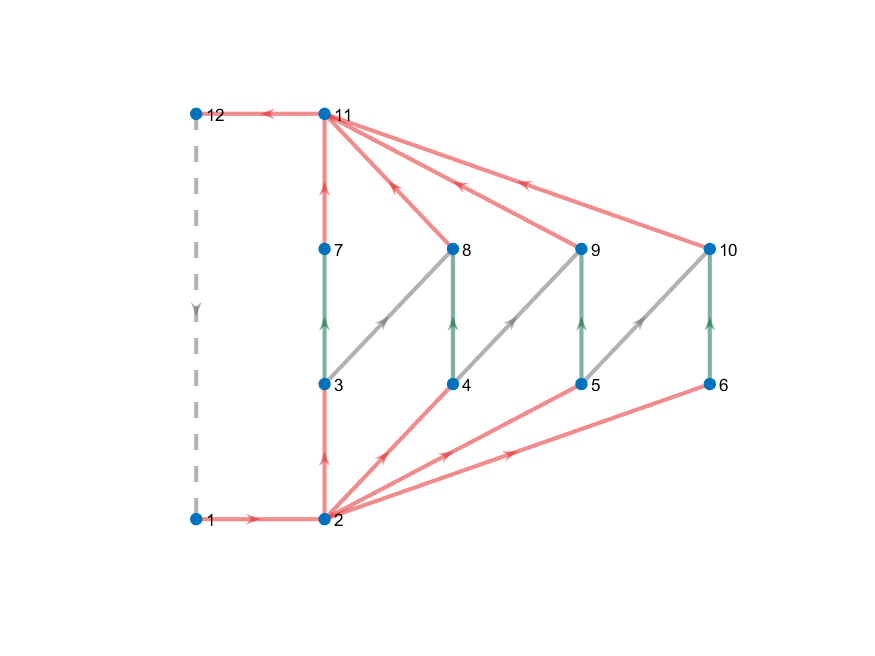
\includegraphics[width=\textwidth]{../attachments/f-dege-mac-4.png}
        \caption{}
        \label{fig:f4-mac}
    \end{subfigure}
    \caption{ 
        RBS structure proposed by Visairo\cite{visairoReconfigurableBatteryPack2008} with 4 batteries. 
        (a) Physical model, (b) graph model, (c) equivalent circuit model, and (d) results obtained by using the proposed method.
        The blue highlighted lines indicate the SPs. 
        The red highlighted lines indicate the open/close states of switches.
        }
    \label{fig:f4-all}
\end{figure}


The reconfigurable architecture proposed by Visairo et al.\cite{visairoReconfigurableBatteryPack2008} is shown in Figure \ref{fig:f4-phy}.
In this architecture, each cell is controlled by about 3 switches on average.
Excepted for two switches ($S_1$ and $S_{13}$ in Figure \ref{fig:f4-phy}) controlling the total circuit, the vertical switches (e.g. $S_2$ and $S_9$ in Figure \ref{fig:f4-phy}) allow the batteries to be directly connected to the main circuit, and the switches($S_6$ for example) in the diagonal direction can realize connecting the batteries in series.
Thus, it can dynamically change the output voltage and current as needed.
The architecture in Figure \ref{fig:f4-phy} only has 4 batteries, but in practice it can add new branches containing batteries and switches to deal with large-scale batteries\cite{kimDependableEfficientScalable2010}.


The graph in Figure \ref{fig:f4-gra} represents a graphical model based on the physical model(Figure \ref{fig:f4-phy}).
The model is presented in the form of a directed graph, capturing the connection relationship between the battery and switch in the circuit.
Vertex 1 and 12 represent the ancode and cathode of the RBS, respectively;
the remaining vertices represent the connection nodes between the batteries and switches.
Battery 1, 2, 3, and 4 are represented by green directed edges in the graph, while switches are represented by gray directed edges with opposite directions.
The external electrical appliance is considered as a directed edge from node 12 to node 1.
In the graph model, the directionality of the edges is strictly specified to ensure that there is no reverse flow of current in the battery and external electrical appliance.


According to Equation \ref{eq:weight}, the weight of the edge corresponding to the battery is the total number of switches, which is 13;
the weight of the edge corresponding to the switch is 1.
By setting the weight in this way, on the one hand, it avoids the simultaneous occurrence of multiple batteries in a single SP, weakening the influence between different batteries;
on the other hand, it minimizes the number of switches on the path, which means that only a few switches (i.e., the switches on the SP) need to be closed to connect the battery to the main circuit.
By using the depth-first search algorithm, the SP of battery 1 can be calculated as the node list $[1, 2, 3, 7, 11, 12]$, and the SPs of the other batteries are shown in Figure \ref{fig:f4-gra}.


The equivalent circuit model, as shows in Figure \ref{fig:f4-circ}, can be obtained based on the assumptions in Section II.
In this model, the batteries and switches are treated as branches, where the battery is regarded as a branch consisting of a voltage source $u_b$ in series with a resistor $r_b$, and the switch is regarded as a branch controlled by a state variable $x_s$ to short or open the circuit.
The branches are represented as direction edges, whose direction is from the node with the smaller number to the larger. 
When the computed current or voltage value is negative, it indicates that the direction of the battery or potential difference is opposite to the preset direction.
Based on the node-edge relationship in Figure \ref{fig:f4-circ}, the incidence matrix $\bm{A}$: can be obtained according to Equation \ref{eq:A}:
{\setlength{\arraycolsep}{2pt}
\begin{equation}
    \begin{array}{cc}
        &  \begin{array}{c c cccc ccccccccccccc} & e_o &e_{b1}  &e_{b2} & e_{b3} & e_{b4} & e_{s1} & e_{s2} & e_{s3} & e_{s4} & e_{s5} & e_{s6} & e_{s7} & e_{s8} & e_{s9} & e_{s10} & e_{s11} & e_{s12} & e_{s13} \end{array}\\
            \begin{array}{c} v_1\\v_2\\v_3\\v_4\\v_5\\v_6\\v_7\\v_8\\v_9\\v_{10}\\v_{11}\\v_{12}\end{array} & \left[
                    \begin{array}{c|cccc|ccccccccccccc}
                        -1  &  0  &  0  &  0  &  0  &  1  &  0  &  0  &  0  &  0  &  0  &  0  &  0  &  0  &  0  &  0  &  0  &  0\\
                        0  &  0  &  0  &  0  &  0  & -1  &  1  &  1  &  1  &  1  &  0  &  0  &  0  &  0  &  0  &  0  &  0  &  0\\
                        0  &  1  &  0  &  0  &  0  &  0  & -1  &  0  &  0  &  0  &  1  &  0  &  0  &  0  &  0  &  0  &  0  &  0\\
                        0  &  0  &  1  &  0  &  0  &  0  &  0  & -1  &  0  &  0  &  0  &  1  &  0  &  0  &  0  &  0  &  0  &  0\\
                        0  &  0  &  0  &  1  &  0  &  0  &  0  &  0  & -1  &  0  &  0  &  0  &  1  &  0  &  0  &  0  &  0  &  0\\
                        0  &  0  &  0  &  0  &  1  &  0  &  0  &  0  &  0  & -1  &  0  &  0  &  0  &  0  &  0  &  0  &  0  &  0\\
                        0  & -1  &  0  &  0  &  0  &  0  &  0  &  0  &  0  &  0  &  0  &  0  &  0  &  1  &  0  &  0  &  0  &  0\\
                        0  &  0  & -1  &  0  &  0  &  0  &  0  &  0  &  0  &  0  & -1  &  0  &  0  &  0  &  1  &  0  &  0  &  0\\
                        0  &  0  &  0  & -1  &  0  &  0  &  0  &  0  &  0  &  0  &  0  & -1  &  0  &  0  &  0  &  1  &  0  &  0\\
                        0  &  0  &  0  &  0  & -1  &  0  &  0  &  0  &  0  &  0  &  0  &  0  & -1  &  0  &  0  &  0  &  1  &  0\\
                        0  &  0  &  0  &  0  &  0  &  0  &  0  &  0  &  0  &  0  &  0  &  0  &  0  & -1  & -1  & -1  & -1  &  1\\
                    \end{array} \right]
    \end{array},
\end{equation}
}
where the rows correspond to vertexes in the graph model, and the first column, second to fourth columns, and last ten columns correspond to external electrical equipment, 4 batteries, and 13 switches, respectively.
According to the above classification of the columns, the matrix $\bm{A}$ can be divided into $\bm{A}_o$, $\bm{A}_b$, and $\bm{A}_s$.


The state matrix $\bm{X}$ is determined by the switches' state, that is, the specific configuration of the RBS.
For example, when switch
$S_1$, $S_2$, $S_3$, $S_4$, $S_5$, $S_9$, $S_{10}$, $S_{11}$, $S_{12}$ and $S_{13}$
are closed, and switch $S_6$, $S_7$ and $S_8$ are open, that is , battery $B_1$, $B_2$, $B_3$ and $_4$ are connected in parallel to supply power to the external circuit, the state matrix $\bm{X}$ is given by
\begin{equation}
    \bm{X} = diag(
    1,
    \underbrace{1,1,1,1}_{\text{batteries}},
    \underbrace{1,1,1,1,1,0,0,0,1,1,1,1,1}_{\text{switches}}
    ).
\end{equation}


When using the algorithm to solve the MAC, one may encounter the situation where the matrix $\bm{Y}_n$ is not full rank, and its inverse matrix cannot directly be obtained.
This is because so many switches are open that some branches with voltage sources are independent of the main circuit and form new circuits.
These circuits have infinite possible values for potential difference between them, since they are not connected to each other.
But the potential of the main circuit, which connects from node 1 to node 12 and completely determines the output, is certain and unique.
Therefore, the non-invertibility of $\bm{Y}_n$ will not affect the final solution.
Here, one can choose the solution where the potential at the node with the smallest number in the independent branch is 0.


\begin{table}[h]
    \caption{Detailed results of the proposed method for the RBS structure proposed by Visairo\cite{visairoReconfigurableBatteryPack2008} with 4 batteries, including the output current, current of each battery, and $\eta$.}
    \label{tab:1}
    \begin{tabular}{ccc}
        \hline
        output current $I_o$       & battery current $\bm{I}_b$       & $\eta$        \\
        \hline\\
        $\displaystyle\frac{4u_b}{4R_o + r_b}$ &  $\displaystyle\left[\frac{u_b}{4R_o + r_b},\frac{u_b}{4R_o + r_b},\frac{u_b}{4R_o + r_b},\frac{u_b}{4R_o + r_b}\right]$   & $4.00$ \\
        \\
        \hline
    \end{tabular}
\end{table}
The final calculation result of $\eta$ for the structure in Figure \ref{fig:f4-phy} is 4.
The corresponding currents of output and each battery are shown in Table \ref{tab:1}.
The corresponding switch control strategy is: $S_1$, $S_2$, $S_3$, $S_4$, $S_5$, $S_9$, $S_{10}$, $S_{11}$, $S_{12}$ and $S_{13}$ are closed (highlighted in red in Figure \ref{fig:f4-mac}), and $S_6$, $S_7$ and $S_8$ are open.
For this structure, when all batteries are connected to the main circuit through the switches in the vertical direction in Figure \ref{fig:f4-phy} and the batteries are connected in parallel, the output current is maximum, which is the sum of the currents of the four batteries.
The MAC of this structure is correctly estimated by our greedy algorithm.


From the specific results of the output current $I_o$ and battery currents $\bm{I}_b$, both are related to the battery voltage $u_b$, internal resistance $r_b$, and external circuit resistance $R_o$.
This means that even for the same structure, the output current will change when the external circuit  or the battery specifications  change.
By dividing the output current by the sum of the battery currents, the obtained $\eta$ does not include items affected by external circuit and batteries.
This characteristic is guaranteed by the linear nature of the RBS circuit.

\subsection{Different structures and sizes}

To further demonstrate the effectiveness of the models and algorithm, RBSs with different structures and sizes are considered.
On the one hand, the modeling and solving of the three battery structures in Figure \ref{fig:arch} are carried out, where the structure in Figure \ref{fig:arch-e} is proposed by Visairo\cite{visairoReconfigurableBatteryPack2008}, the structure in Figure \ref{fig:arch-f} is proposed by Lawson\cite{lawsonSoftwareConfigurableBattery2012}, and the structure in Figure \ref{fig:arch-ef} is a combination of the two. All three structures have 4 battery cells.
On the other hand, the modeling and solving of the battery structures proposed by Visairo\cite{visairoReconfigurableBatteryPack2008} with different numbers of battery cells (2, 4, and 6 cells) are also carried out.

The greedy algorithm provided accurate estimates of the structure MAC and generated safe and effective switch control strategies, as indicated by the results shown in Figure \ref{fig:d-structure} and \ref{fig:d-size}, where the highlighted red switches denote the closed positions.
Furthermore, the results about currents in Table \ref{tab:d-structure} and \ref{tab:d-size} show that the output currents are influenced by the external circuit resistance, battery potential, and internal resistance, but are linearly related to the battery currents, consistent with the conclusion about $\eta$ in the previous subsection.

\begin{figure}[htbp]
    \centering
    \begin{subfigure}[b]{0.45\textwidth}
        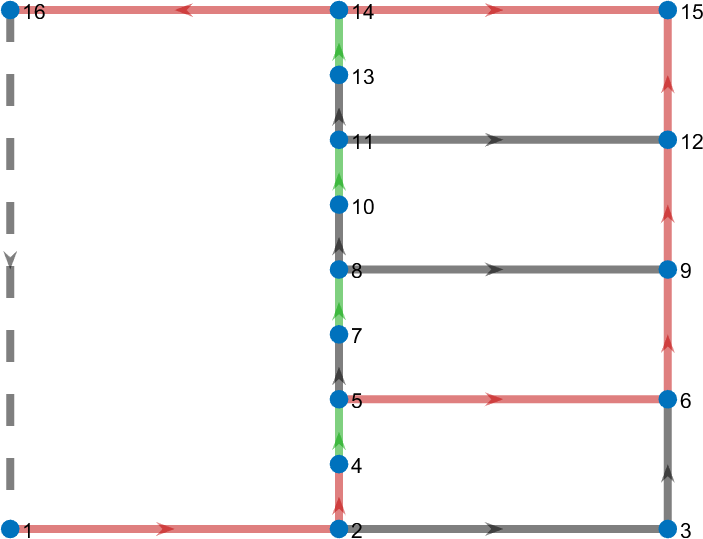
\includegraphics[width=\textwidth]{../attachments/e-dege-mac-4.png}
        \caption{}
        \label{fig:d-structure-f4}
    \end{subfigure}
    \hspace{0.05\textwidth}
    \begin{subfigure}[b]{0.45\textwidth}
        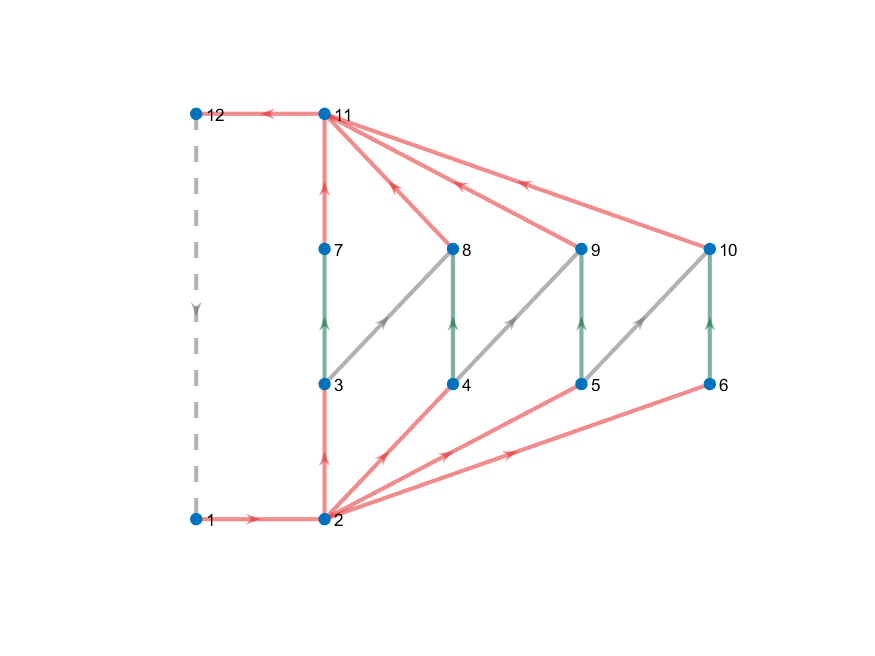
\includegraphics[width=\textwidth]{../attachments/f-dege-mac-4.png}
        \caption{}
        \label{fig:d-structure-e4}
    \end{subfigure}
    \hspace{0.05\textwidth}
    \begin{subfigure}[b]{0.45\textwidth}
        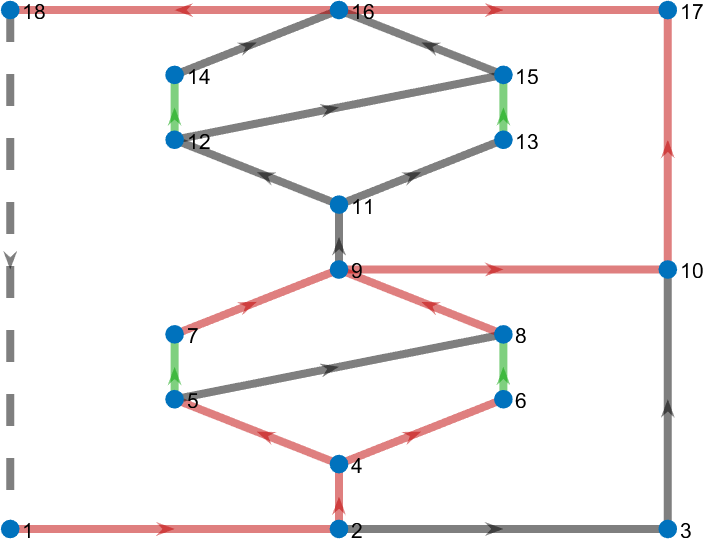
\includegraphics[width=\textwidth]{../attachments/e2f2-dege-mac.png}
        \caption{}
        \label{fig:d-structure-e2f2}
    \end{subfigure}
    \caption{
        The switches state when the output current is MAC on structure (a) proposed by Lawson\cite{lawsonSoftwareConfigurableBattery2012}, (b) proposed by Visairo\cite{visairoReconfigurableBatteryPack2008}, and (c) combining  Lawson's and Visairo's structure. 
        The red highlighted lines indicate the open/close states of switches.
        }
    \label{fig:d-structure}
\end{figure}

\begin{table}[h]
    \centering
    \caption{
        detailed results of the proposed method for the RBS with 4 batteries (a) proposed by lawson\cite{lawsonSoftwareConfigurableBattery2012}, (b) proposed by  visairo\cite{visairoReconfigurableBatteryPack2008} and (c) combining both  , including the output current, current of each battery, and $\eta$.}
    \label{tab:d-structure}
    \begin{tabular}{cccc}
        \hline
        structure &  output current $I_o$       & battery current $\bm{I}_b$       & $\eta$        \\
        \hline\\
        Lawson\cite{lawsonSoftwareConfigurableBattery2012} &  $\displaystyle\frac{u_b}{R_o + r_b}$ &  $\displaystyle\left[\frac{u_b}{R_o + r_b},0,0,0\right]$   & $1.00$ \\
        \\
        Visairo\cite{visairoReconfigurableBatteryPack2008} &  $\displaystyle\frac{4u_b}{4R_o + r_b}$ &  $\displaystyle\left[\frac{u_b}{4R_o + r_b},\frac{u_b}{4R_o + r_b},\frac{u_b}{4R_o + r_b},\frac{u_b}{4R_o + r_b}\right]$   & $4.00$ \\
        \\
        combining both &  $\displaystyle\frac{2u_b}{2R_o + r_b}$ &  $\displaystyle\left[\frac{u_b}{2R_o + r_b},\frac{u_b}{2R_o + r_b},0,0\right]$   & $2.00$ \\
        \\
        \hline
    \end{tabular}
\end{table}

\begin{figure}[htbp]
    \centering
    \begin{subfigure}[b]{0.45\textwidth}
        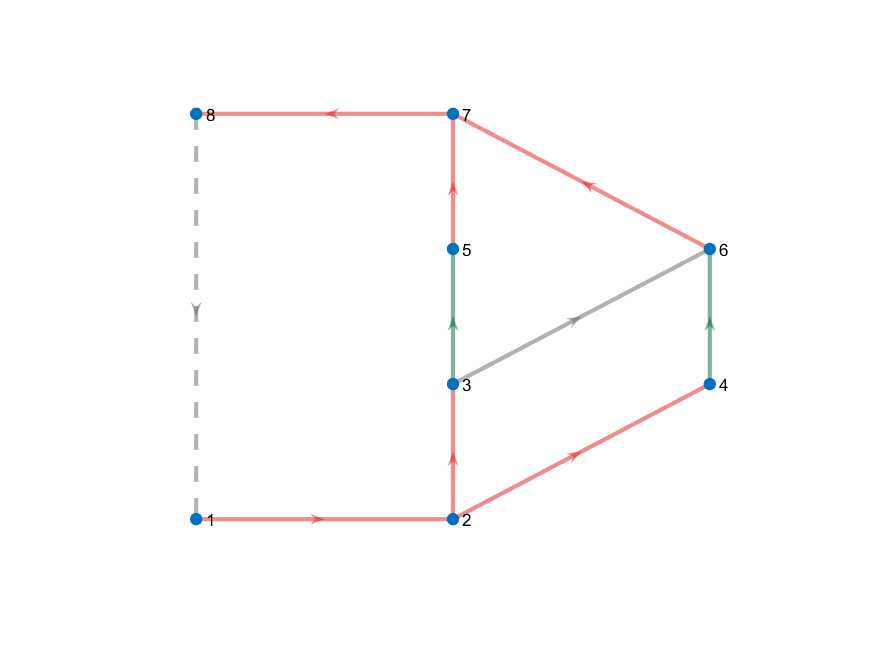
\includegraphics[width=\textwidth]{../attachments/f-dege-mac-2.png}
        \caption{}
        \label{fig:d-size-2}
    \end{subfigure}
    \hspace{0.05\textwidth}
    \begin{subfigure}[b]{0.45\textwidth}
        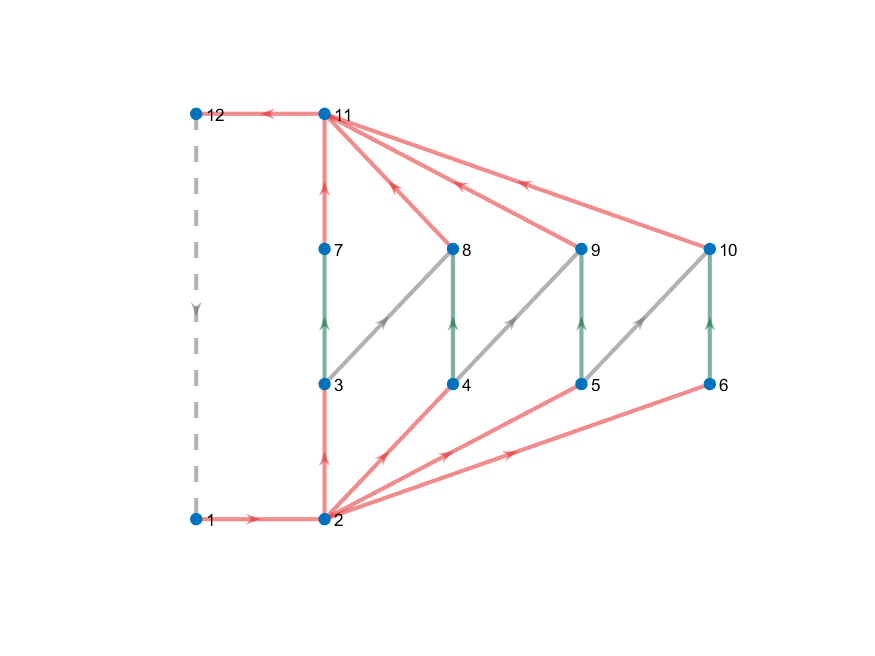
\includegraphics[width=\textwidth]{../attachments/f-dege-mac-4.png}
        \caption{}
        \label{fig:d-size-4}
    \end{subfigure}
    \hspace{0.05\textwidth}
    \begin{subfigure}[b]{0.45\textwidth}
        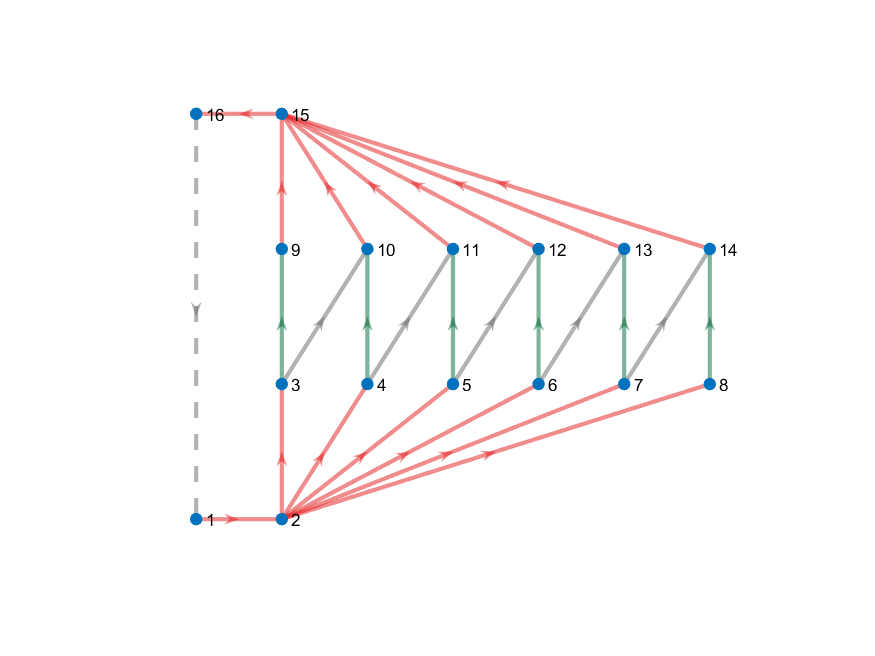
\includegraphics[width=\textwidth]{../attachments/f-dege-mac-6.png}
        \caption{}
        \label{fig:d-size-6}
    \end{subfigure}
    \caption{
        The switches state when the output current is MAC on structure proposed by Visairo\cite{visairoReconfigurableBatteryPack2008} with (a)2, (b)4 and (c) 6 batteries.  
        The red highlighted lines indicate the open/close states of switches.
        }
    \label{fig:d-size}
\end{figure}

\begin{table}[h]
    \caption{detailed results of the proposed method for the RBS proposed by visairo\cite{visairoReconfigurableBatteryPack2008} with (a)2, (b)4 and (c) 6 batteries , including the output current, current of each battery, and $\eta$.}
    \label{tab:d-size}
    \begin{tabular}{cccc}
        \hline
        size &  output current $I_o$       & battery current $\bm{I}_b$       & $\eta$        \\
        \hline\\
        2 &  $\displaystyle\frac{2u_b}{2R_o + r_b}$ &  $\displaystyle\left[\frac{u_b}{2R_o + r_b},\frac{u_b}{2R_o + r_b},\frac{u_b}{2R_o + r_b},\frac{u_b}{2R_o + r_b}\right]$   & $2.00$ \\
        \\
        4 &  $\displaystyle\frac{4u_b}{4R_o + r_b}$ &  $\displaystyle\left[\frac{u_b}{4R_o + r_b},\frac{u_b}{4R_o + r_b},\frac{u_b}{4R_o + r_b},\frac{u_b}{4R_o + r_b}\right]$   & $4.00$ \\
        \\
        6 &  $\displaystyle\frac{6u_b}{6R_o + r_b}$ &  $\displaystyle\left[\frac{u_b}{6R_o + r_b},\frac{u_b}{6R_o + r_b},\frac{u_b}{6R_o + r_b},\frac{u_b}{6R_o + r_b}\right]$   & $6.00$ \\
        \\
        \hline
    \end{tabular}
\end{table}

\section{Conclusion}

A graph model and a circuit model were developed, and a greedy strategy was employed to solve the MAC. 
The proposed method was tested on RBSs of varying structures and sizes. 
Additionally, an indicator, denoted by $\eta$ , was introduced to evaluate the performance of the RBS's output current. 
This work presents an effective approach for designing and evaluating the output current performance of RBS. 
Future research could focus on developing new performance indicators for evaluating RBS performance using the currents and voltages obtained by this method, as well as modifying the equivalent model of the battery to enable more accurate simulations of RBS, including transient analysis.

\section{Appendix}
\begin{algorithm}
    \caption{Get the max available currents of a certain RBS}\label{alg:eta_RBS}
    \KwData{Directed graph model $G(V,E)$ of the RBS}
    \KwResult{$\max \eta$}
    \For{$i \in E_b$}{
        $P_i \leftarrow \{path| \text{starts at $v_1$ and ends at $v_n$} \}$\;
        $SP_i \leftarrow p_i \text{ which has the minimum}~\omega(p_i)~\text{among all}~p_i \in P_i. $
    }
    get $\bm{A}$ by Equation \ref{eq:A}\;
    \While{not yet determine $\max \eta$ }
    {
        $N_{sel} \leftarrow \text{number of selected $SP$s calculated by dichotomy}$\;
        $C_b    \leftarrow \text{set of all combinations of $N_{sel} $~batteries from $N_b$}$\;
        \For{$c_b \in C_b$}{
            $\bm{x}_s \leftarrow \text{list of all switches' state: $x_s[j]=1$ if $ j \in \bigcup_{i\in c_b}SP_i $ else 0}$\;
            $\bm{X} \leftarrow diag[1,1,\cdots,1,\bm{x}_s] $\;
            get $\bm{Y}_n$ by Equation \ref{eq:Yn}\;
            \eIf{$\bm{Y}_n$ is invertible}{
            }{construct an effective solution}
            get $I_o$ by Equation \ref{eq:I_o}\;
            get $\bm{I}_b$ by Equation \ref{eq:I_b}\;
            \eIf{$\max(\bm{I}_b)\leq I_m$}{
                $\eta \leftarrow I_o/\max(\bm{I}_b)$\;
            }{break}
        }
    }
\end{algorithm}

\bibliographystyle{ieeetr}
\bibliography{../attachments/my_ref}

\end{document}
